\documentclass[10pt]{article}
\usepackage{graphicx}
\usepackage[margin=1.5cm]{geometry}
\usepackage{amsmath}
\def\brcurs{{\mbox{$\resizebox{.16in}{.08in}{
\includegraphics{BoldR}}$}}}
\def\rcurs{{\mbox{$\resizebox{.16in}{.08in}{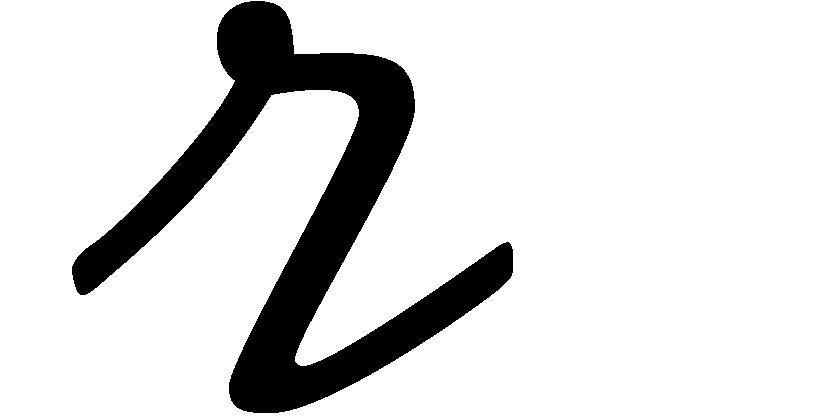
\includegraphics{ScriptR}}$}}}

\begin{document}
\twocolumn

\title{Tuesday Warm-up: Electrostatics}
\author{Prof. Jordan C. Hanson}

\maketitle

\section{Memory Bank}

\begin{itemize}
\item Definition of electric field: $\mathbf{F} = q\mathbf{E}$.
\item Permittivity of free space: $\epsilon_0 = 8.85 \times 10^{-12}$ N$^{-1}$C$^2$m$^{-2}$
\item Let $\rho(\mathbf{r}')$ represent the charge density.
\item Let $Q_{\rm enc} = \int \rho d\tau'$, the total charge within a volume.
\item Coulomb's Law, discrete
\begin{equation}
\mathbf{E}(\mathbf{r}) = \frac{1}{4\pi\epsilon_0}\sum_i \frac{q_i}{\rcurs_i^2}\hat{\brcurs}
\end{equation}
\item Coulomb's Law, continuous
\begin{equation}
\mathbf{E}(\mathbf{r}) = \frac{1}{4\pi\epsilon_0}\int \frac{\rho(\mathbf{r}')}{\rcurs^2}\hat{\brcurs}d\tau'
\end{equation}
\item Gauss' Law, integral form
\begin{equation}
\oint \mathbf{E} \cdot d\mathbf{a} = \frac{1}{\epsilon_0}Q_{\rm enc}
\end{equation}
\item Gauss' Law, differential form
\begin{equation}
\nabla \cdot \mathbf{E} = \frac{1}{\epsilon_0}\rho
\end{equation}
\item Definition of potential
\begin{equation}
V(\mathbf{r}) = - \int_{\rm \mathcal{O}}^{\mathbf{r}} \mathbf{E}(\mathbf{r}') \cdot d\mathbf{l}'
\end{equation}
\item Relationship between potential and field:
\begin{equation}
\mathbf{E} = -\nabla V
\end{equation}
\end{itemize}

\begin{figure}
\centering
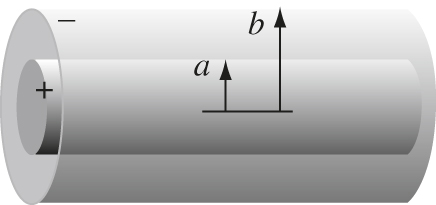
\includegraphics[width=0.3\textwidth]{figures/2_26.jpg}
\caption{\label{fig:1} A positively charged cylinder with charge density $+\rho$, and a negatively charged cylindrical shell with charge density $-\sigma$.}
\end{figure}

\section{Gauss' Law}

\begin{enumerate}
\item A long coaxial cable (Fig. \ref{fig:1}) carries a uniform volume charge density $+\rho$ on the inner cylinder (radius $a$), and a uniform surface charge density $-\sigma$ on the outer cylindrical shell (radius $b$).  The cable as a whole is electrically neutral.  Find the electric field in each of the following three regions: (i) inside the inner cylinder, (ii) between the cylinders, and (iii) outside the cable.  Plot $|\mathbf{E}|$ as a function of $r$.  \\ \vspace{4cm}
\end{enumerate}

\section{The Curl of $\mathbf{E}$}

\begin{enumerate}
\item Using Stoke's Theorem, show that the curl of the following vector field is zero:
\begin{equation}
\mathbf{v} = \frac{\hat{r}}{r^2}
\end{equation} \vspace{2cm}
\item Show that the potential of a point charge $q$ at the origin is 
\begin{equation}
V(r) = \frac{1}{4\pi\epsilon_0}\frac{q}{r}
\end{equation}
\end{enumerate}

\end{document}
